\documentclass[../../thesis.tex]{subfiles}

\graphicspath{{Figures/}}

\begin{document} 
\chapter{Cross-Spectra analysis and Cosmological parameters} \label{chap:xspectrum}

\ifSubfilesClassLoaded{
    \tableofcontents
}{
    \minitoc
}

\section*{Introduction}

The previous chapters focused on map-domain approaches to the analysis of QUBIC observations. In particular, the Frequency Map-Making (FMM) algorithm provides a set of reconstructed frequency maps, while the Component Map-Making (CMM) framework performs component separation directly during the map reconstruction process. However, we have not yet described how component separation can be performed using frequency maps alone. This is achieved through the widely used \emph{cross-spectrum analysis} method.
This approach relies on the spectral behaviour of the observed sky. Since the Cosmic Microwave Background (CMB), thermal dust, synchrotron emission, and other astrophysical foregrounds exhibit distinct frequency dependencies, their contributions can be statistically disentangled by exploiting the correlations between maps observed at different frequencies. Rather than reconstructing individual component maps, the analysis is performed directly on the angular power spectra and cross-spectra derived from the reconstructed frequency maps.
Cross-spectrum methods offer several advantages. First, they naturally suppress noise biases when independent noise realizations are available, typically through dedicated simulations. Second, they provide a flexible framework for modelling astrophysical foregrounds and instrumental effects directly at the statistical level. Finally, they establish a direct connection between the measured observables and the theoretical predictions of cosmological models.

The objective of this chapter is therefore twofold. The first part presents the construction and modelling of the multi-frequency angular power spectra obtained from FMM frequency maps, together with the methodology used to separate the different astrophysical contributions. The second part describes how these spectra can be used to constrain cosmological parameters, with particular emphasis on the tensor-to-scalar ratio $r$, which constitutes the primary scientific target of QUBIC.

\personal{The cross-spectrum component separation framework and the associated cosmological parameter estimation pipeline were originally developed jointly with Mathias Regnier for the methodological studies presented in \cite{FMM,CMM}, as well as for his PhD thesis. During the second and third years of my PhD, I significantly extended these tools by improving their generality, software architecture, and integration within the QUBIC simulation and reconstruction framework. I also automated large parts of the analysis pipeline, enabling the production of end-to-end forecasts with minimal manual intervention.}

\section{Cross-Spectrum component separation}

\subsection{General Principle}

The general idea of cross-spectrum analysis is to compare angular cross-power spectra between frequency maps in order to constrain both foreground and CMB parameters. Given a physical emission model for each astrophysical component, one can derive its associated angular power spectrum and its frequency dependence, and thus predict the corresponding cross-spectra. The availability of multiple frequency channels improves the constraints on these parameters, making this approach particularly well suited to QUBIC, which can reconstruct multiple sub-bands within its bandwidth through spectral imaging.

\subsubsection{Cross-spectra model}

For a sky composed of CMB, thermal dust, and synchrotron emission, the cross-spectrum between two frequency maps at $\nu_1$ and $\nu_2$ can be written as the sum of the individual contributions:

\begin{equation}
    \begin{split}
        \mathcal{D}_{\ell}^{\nu_1 \times \nu_2} &= \mathcal{D}_{\ell, CMB}^{\nu_1 \times \nu_2} + \mathcal{D}_{\ell, Dust}^{\nu_1 \times \nu_2} + \mathcal{D}_{\ell, Sync}^{\nu_1 \times \nu_2} + \mathcal{D}_{\ell, Dust\times Sync}^{\nu_1 \times \nu_2} \\
        &= r \times \mathcal{D}_{\ell}^{\text{tensor}} + A_{\text{lens}} \times \mathcal{D}_{\ell}^{\text{lensed}} \\
        &+ A_d \Delta_d f_d^{\nu_1}(\beta_d, T_d) f_d^{\nu_2}(\beta_d, T_d) \left( \frac{\ell}{\ell_0} \right)^{\alpha_d} + A_s \Delta_s f_s^{\nu_1}(\beta_s, T_s) f_s^{\nu_2, T_s}(\beta_s, T_s) \left( \frac{\ell}{\ell_0} \right)^{\alpha_s} \\
        &+ \varepsilon \sqrt{A_d A_s} \left( f_d^{\nu_1}(\beta_d, T_d) f_s^{\nu_2}(\beta_s, T_s) + f_s^{\nu_1}(\beta_s, T_s) f_d^{\nu_2}(\beta_d, T_d)\right) \left( \frac{\ell}{\ell_0} \right)^{\frac{\alpha_d + \alpha_s}{2}}.
    \end{split}
\label{eq: MCT_eq}
\end{equation}

This expression combines the contributions of the CMB (tensor and lensed scalar modes), thermal dust, and synchrotron emission, as well as a possible spatial correlation term between dust and synchrotron components. Each foreground contribution depends on its spectral energy distribution $f_{\mathrm{comp}}^{\nu}(\beta_{\mathrm{comp}})$, as introduced in Section~\ref{section:foregrounds}, and is normalised at a reference multipole $\ell_0$, typically set to $80$~\cite{Krachmalnicoff_2016}.

The CMB contribution depends on two parameters: the tensor-to-scalar ratio $r$, which is the primary scientific target of QUBIC, and the gravitational lensing amplitude $A_{\mathrm{lens}}$. In the simulations, $r$ is set to zero, while $A_{\mathrm{lens}}$ is fixed to unity, since QUBIC is not expected to have sufficient sensitivity to constrain lensing effects (see subsection~\ref{sub:lensing}).
The thermal dust component depends on several parameters. These include the dust amplitude $A_d$, defined at a reference frequency $\nu_{0,d} = 353,\mathrm{GHz}$, corresponding to the most dust-dominated Planck channel; the angular power-law index $\alpha_d$; the spectral index $\beta_d$; the dust temperature $T_d$; and the frequency decorrelation parameter $\Delta_d$. Following \cite{Planck2018XI}, the dust temperature is fixed to $T_d = 20,\mathrm{K}$ and the spectral index to $\beta_d = 1.54$. In addition, the decorrelation parameter $\Delta_d$ is not independently fitted, as it is fully degenerate with the amplitude $A_d$.
The synchrotron component is described by an analogous set of parameters, with a reference frequency fixed at $\nu_{0,s} = 23,\mathrm{GHz}$. It is characterized by its amplitude $A_s$, spectral index $\beta_s$, angular power-law index $\alpha_s$, and frequency decorrelation parameter $\Delta_s$, following the same formalism as for dust.
Finally, the spatial correlation between dust and synchrotron emissions is parametrised by $\varepsilon$.

\subsubsection{Cross-spectra computation}

The cross-spectra are computed from the reconstructed frequency maps using the \emph{NaMaster} package~\cite{alonso2019}\footnote{\url{https://github.com/LSSTDESC/NaMaster}}, which is widely used for pseudo-$C_\ell$ estimation in CMB analyses. The angular power spectra are estimated from HEALPix~\cite{healpix2005} maps with a resolution parameter $N_{\mathrm{side}} = 256$.
The multipole range considered extends from $\ell_{\mathrm{min}} = 40$ to $\ell_{\mathrm{max}} = 2N_{\mathrm{side}} - 1 = 511$, with a constant bin width $\Delta_\ell$. The upper limit is imposed by the pseudo-$C_\ell$ estimator implemented in NaMaster, whose accuracy degrades for polarisation maps at multipoles significantly larger than $2N_{\mathrm{side}}$. The lower limit is determined by the QUBIC instrumental response. Indeed, the sensitivity of a bolometric interferometer decreases at angular scales larger than the separation between the peaks of the synthesized beam, resulting in a reduced sensitivity to multipoles below $\ell \simeq 40$~\cite{QUBICI}. Finally, the binning parameter $\Delta_\ell$ was determined empirically as a compromise between spectral resolution and statistical uncertainty. Larger bins reduce the variance of the estimated spectra, while smaller bins preserve more information on their multipole dependence.

\subsection{Noise debiasing}

The power spectrum of the reconstructed maps can be written as the sum of the signal power spectrum, noted $S_\ell$, and the noise power spectrum, $N_\ell$. To remove the bias introduced by $N_\ell$ during the parameters' estimation, we will perform multiple end-to-end simulations while varying the noise seed. 
Then, we compute the average cross-power spectrum of the reconstructed maps $\overline{D_\ell^{\nu_1 \times \nu_2}}$ and the average cross-power spectrum of the residual maps, which is equivalent to $\overline{N_\ell^{\nu_1 \times \nu_2}}$. By simply computing the difference between the two, we can compute the unbiased cross-power spectrum of the signal $\overline{S_\ell^{\nu_1 \times \nu_2}} \equiv \overline{D_\ell^{\nu_1 \times \nu_2}} - \overline{N_\ell^{\nu_1 \times \nu_2}}$. The Figure \ref{fig:xspectra_unbiasing} shows the unbiasing process. The orange points are $\overline{D_\ell^{\nu_1 \times \nu_2}}$, with contribution from sky signals and noise bias, while blue points is the unbiased cross-sepctra $\overline{S_\ell^{\nu_1 \times \nu_2}}$. We also added the theoritical model for cross-power spectra, based on equation \ref{eq: MCT_eq} for a sky composed of Dust and CMB, with the red dashed line.

\begin{figure}[!htbp]
    \begin{minipage}{0.5\linewidth}
        \centerline{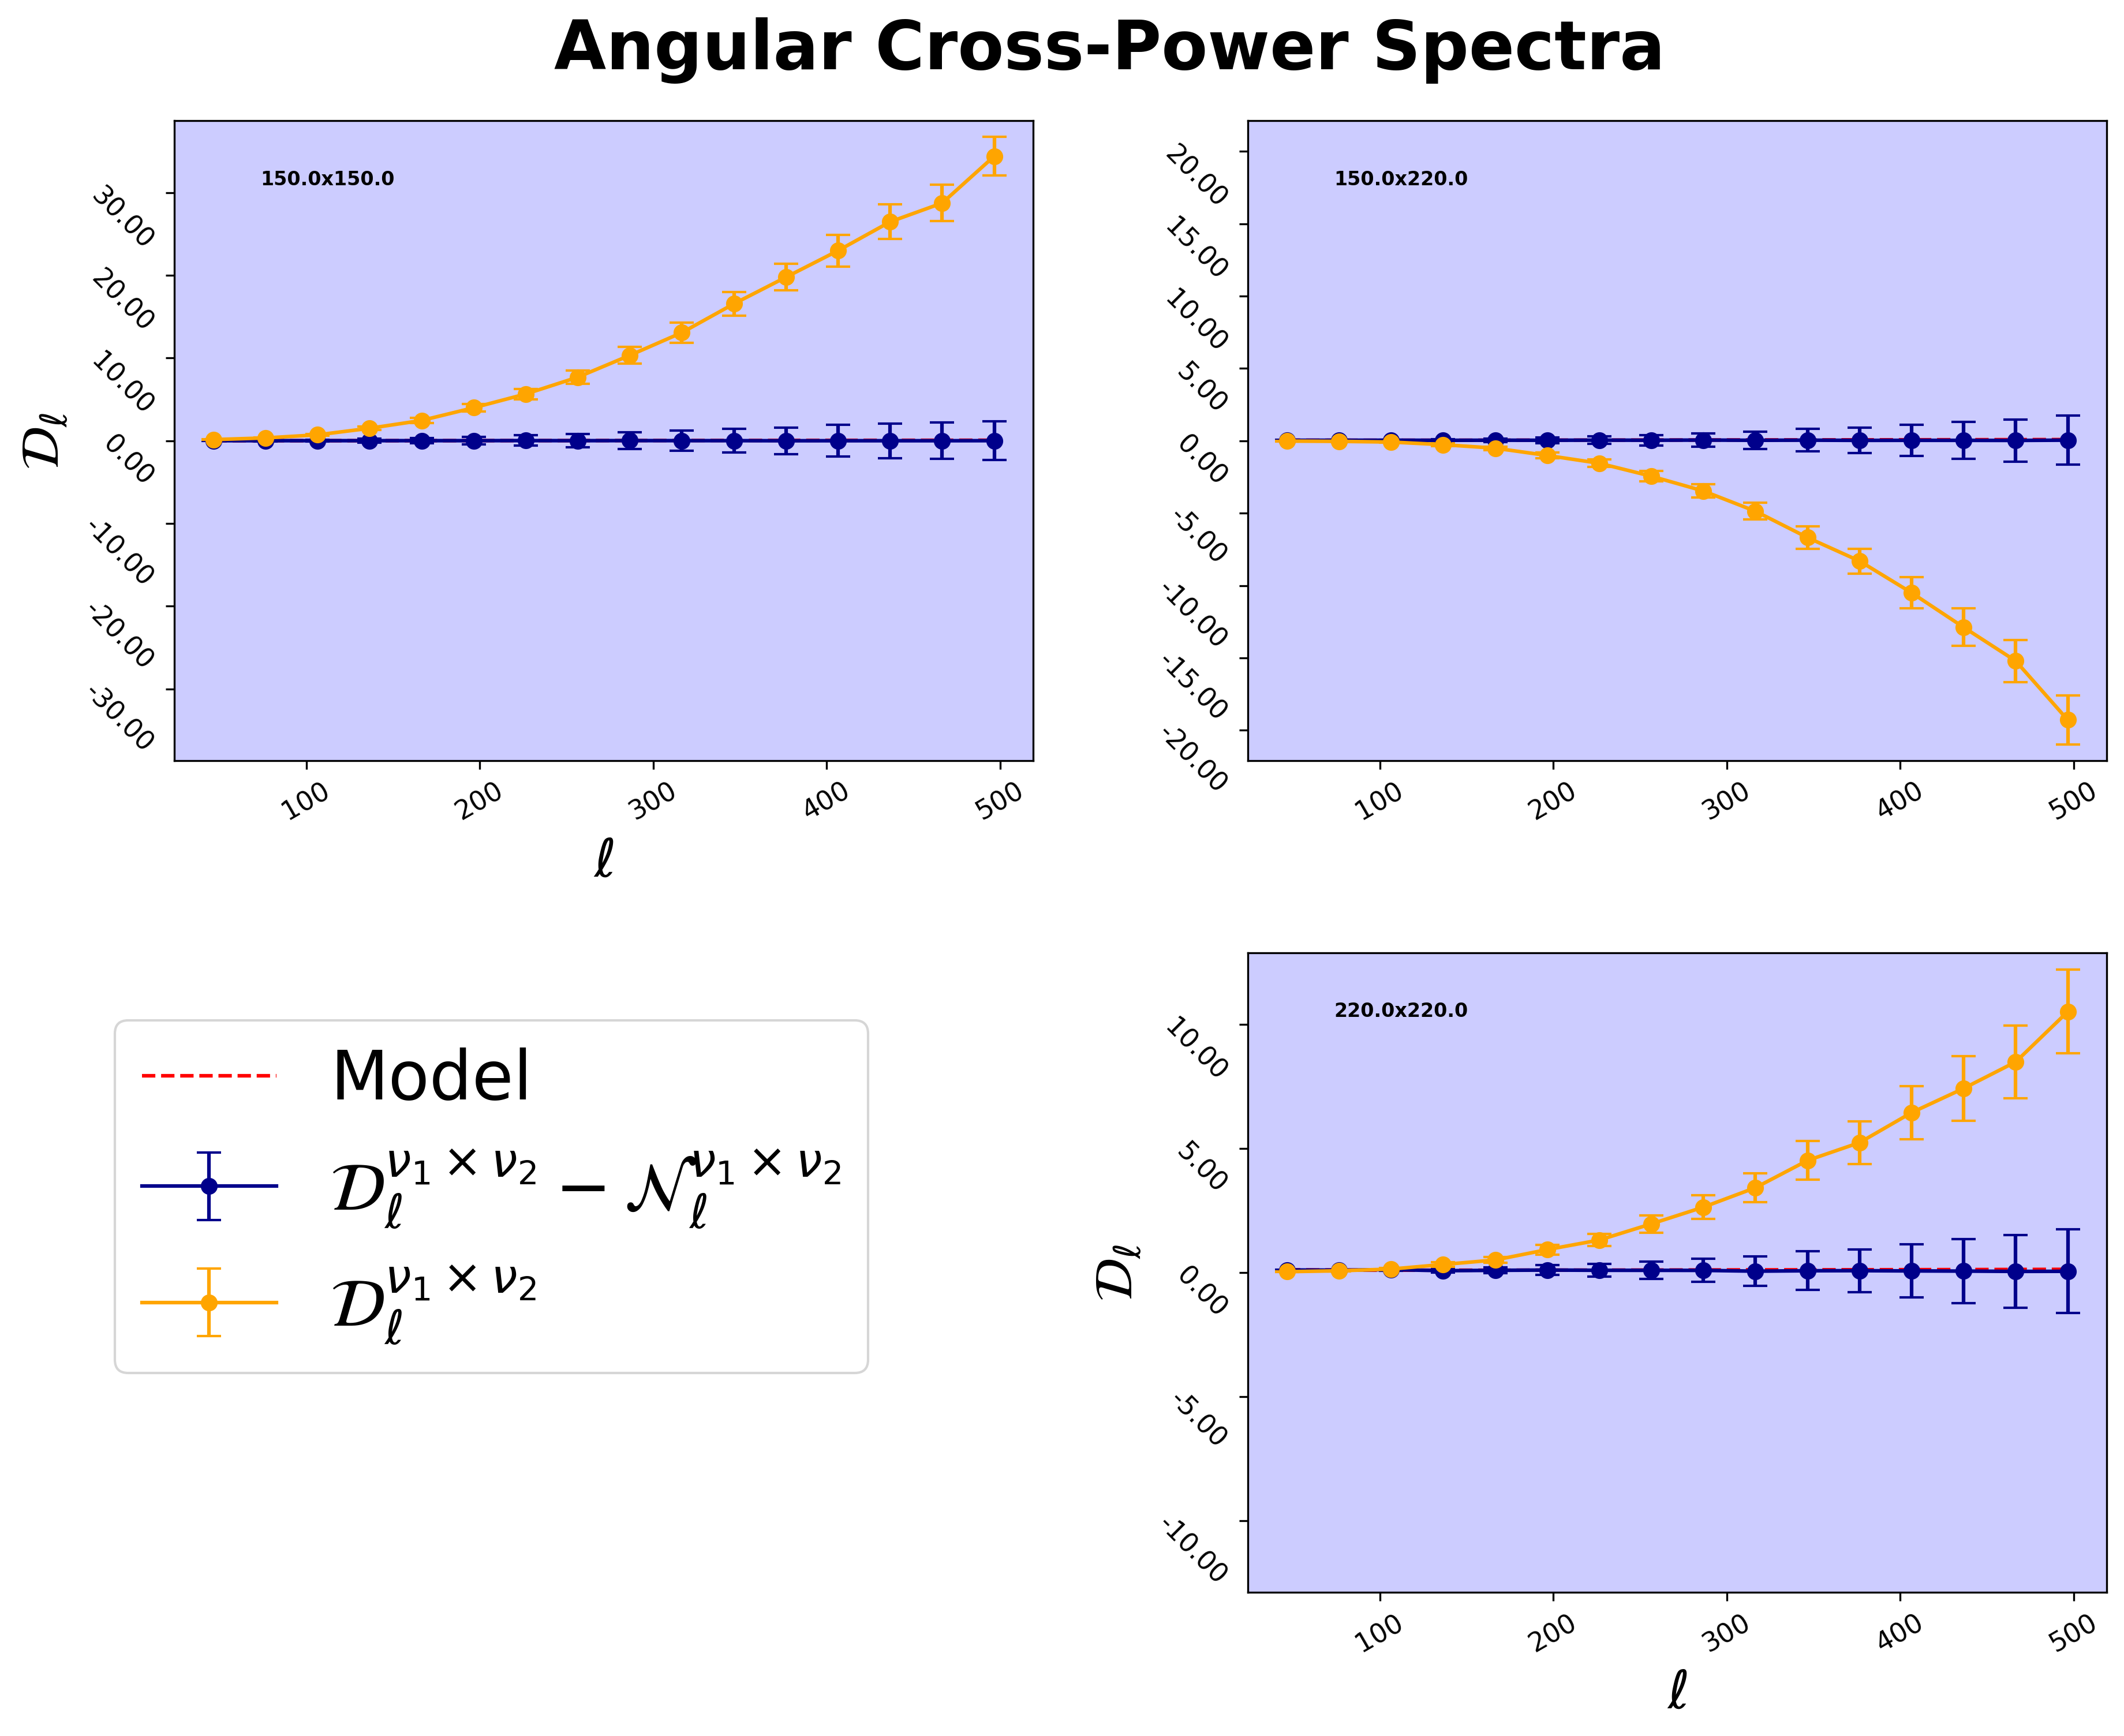
\includegraphics[width=1\linewidth]{xspectra_unbiasing_w_noise.png}}
    \end{minipage}
    \hfill
    \begin{minipage}{0.5\linewidth}
        \centerline{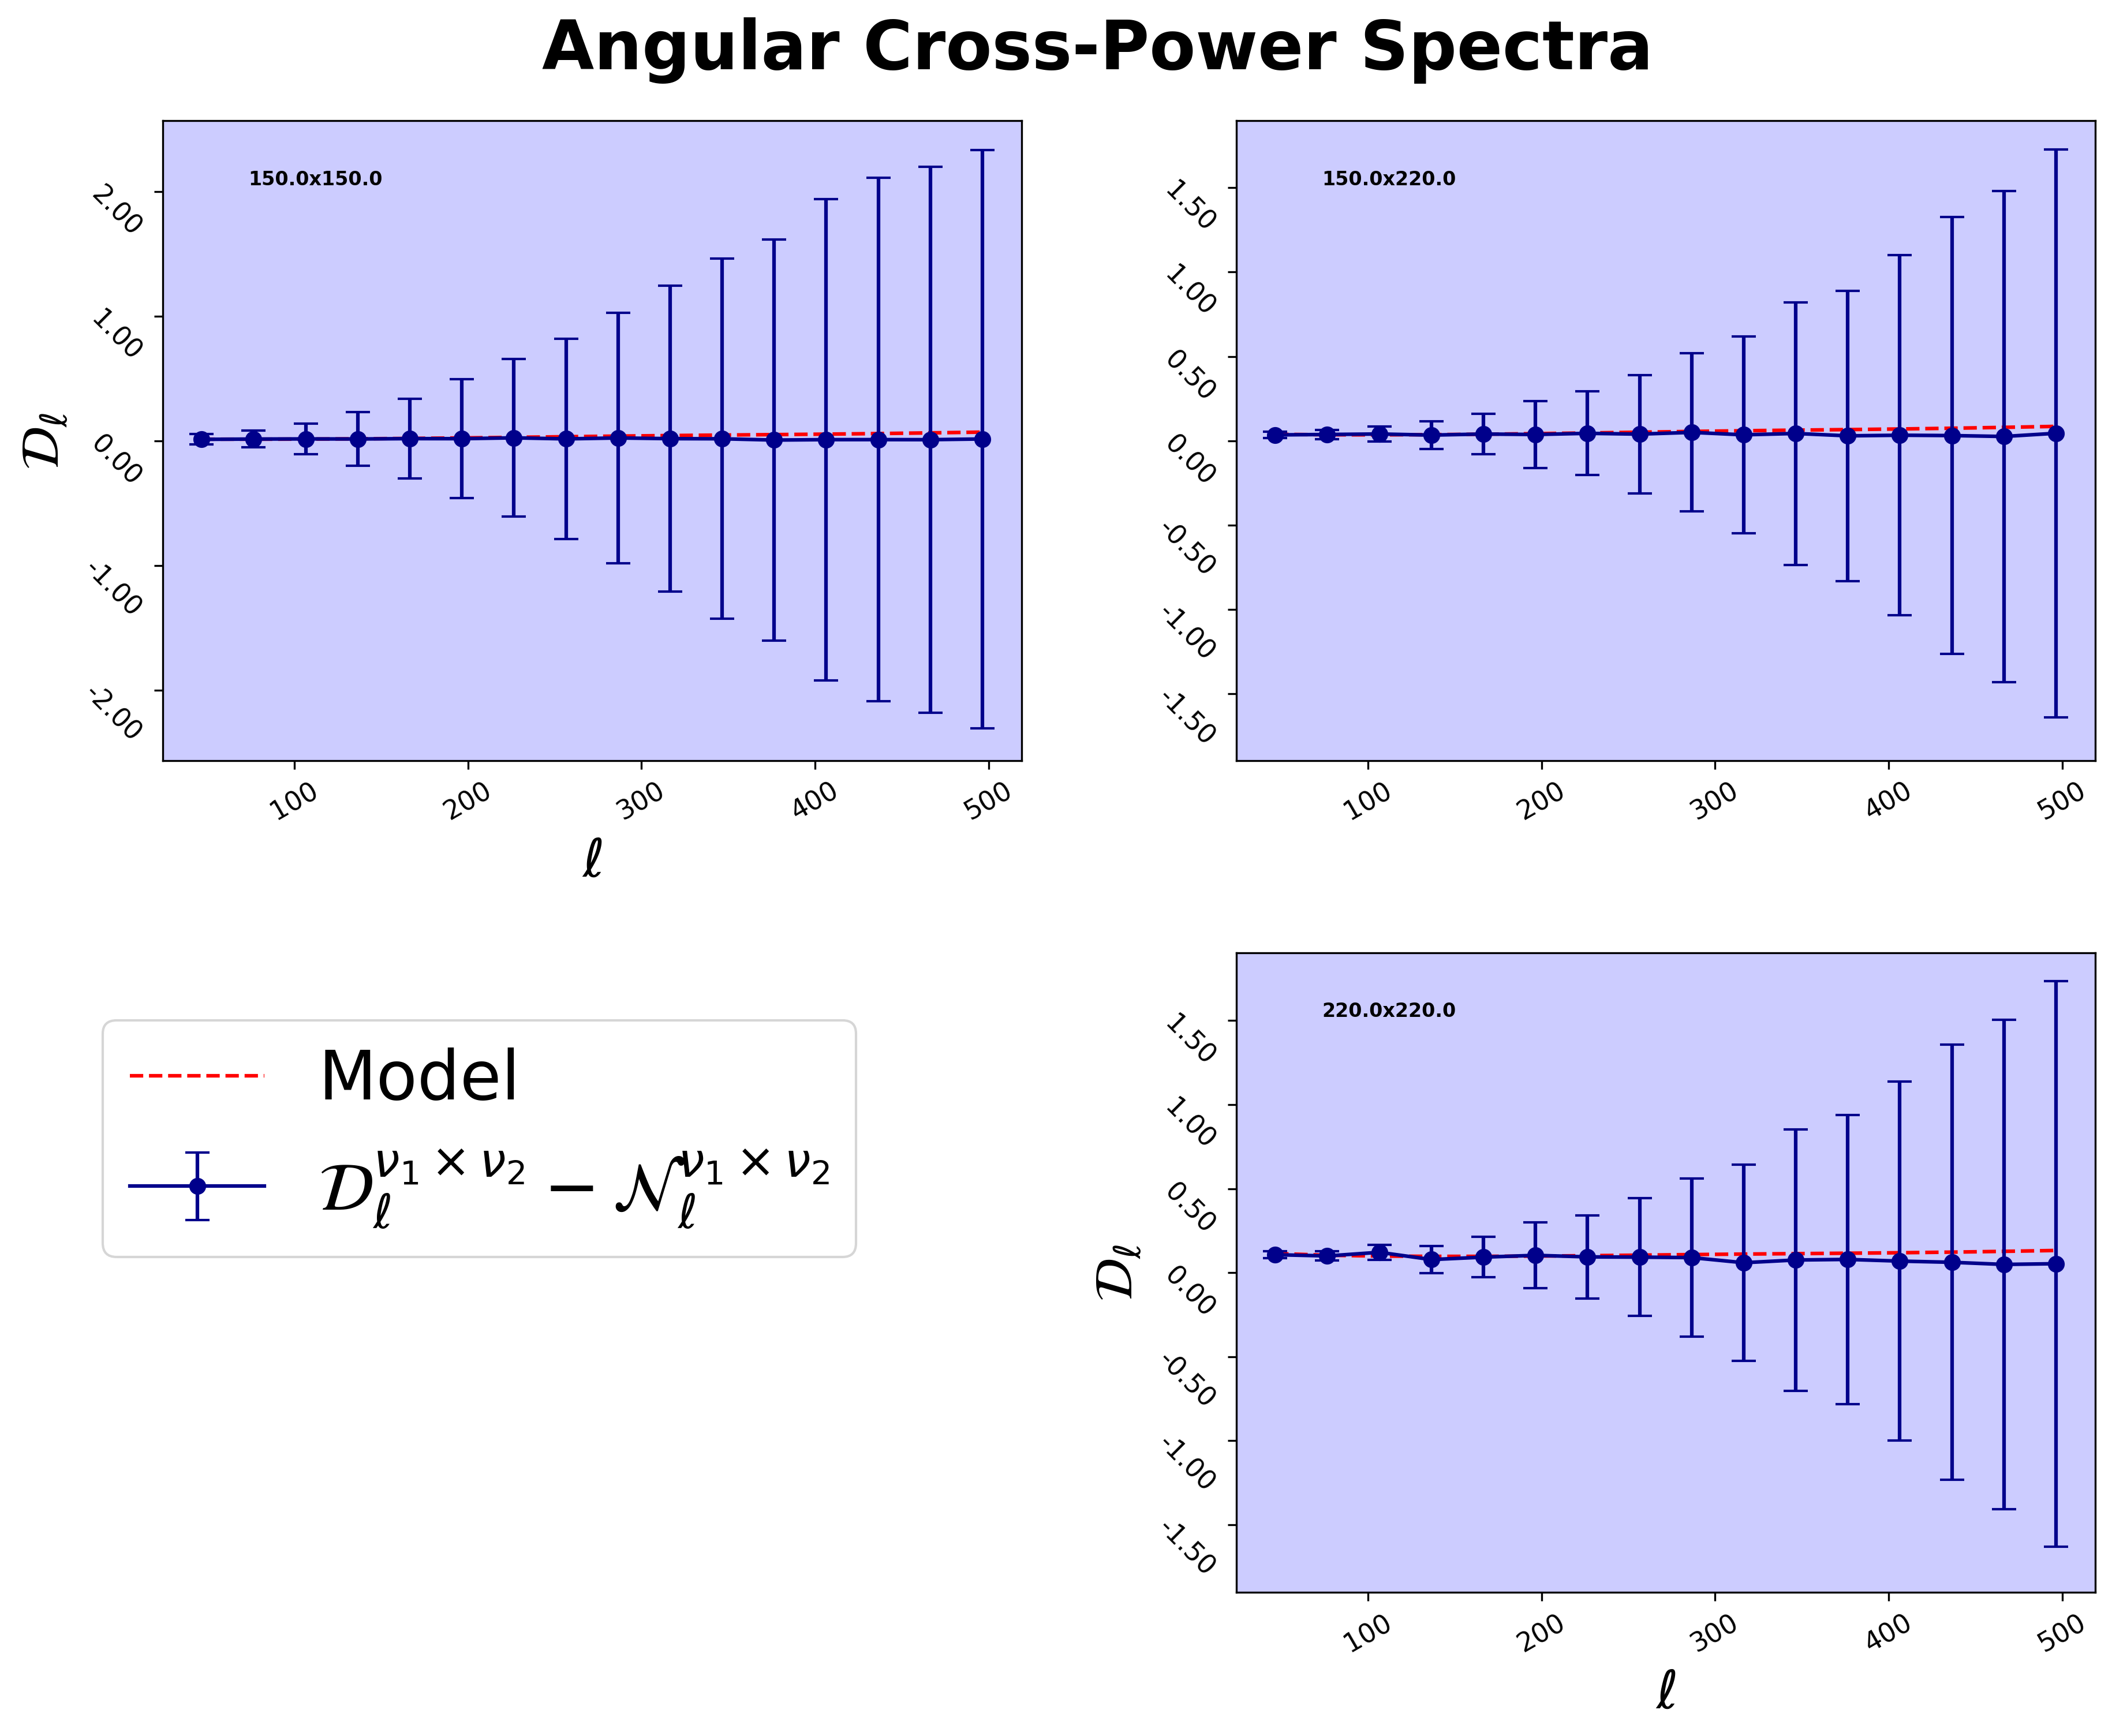
\includegraphics[width=1\linewidth]{xspectra_unbiasing_wo_noise.png}}
    \end{minipage}
    \caption{}
    \label{fig:xspectra_unbiasing}
\end{figure}



\subsection{Noise covariance matrix}

\section{Cosmological parameters' estimation}

\rmk{Should be in forecast chapter ?}

\subsection{FMM cross-spectrum}

\subsection{CMM cross-spectrum}

\end{document}